\documentclass[landscape]{article}

%%%%%%%%%%%%%%%%%%%%%%%%%%%%%%%%%
% PACKAGES
%%%%%%%%%%%%%%%%%%%%%%%%%%%%%%%%%

\usepackage{acronym,amsthm,babel,boxedminipage,longtable,fancyhdr,framed, mathtools,amsmath, amssymb,
  colortbl,epsfig,lscape,multirow,setspace,tabularx,titlesec,subcaption,graphicx,%tweaklist,
  moreverb,xcolor,xspace}

\usepackage[
bookmarks,bookmarksopen,bookmarksnumbered,bookmarksopenlevel=2,
pdftitle=Streaming\ NMT\ from\ EU\ languages\ to\ English,%
citebordercolor=blue,
filebordercolor=teal,
linkbordercolor=lightgray,
menubordercolor=violet,
urlbordercolor=lightgray,
runbordercolor=darkgray]{hyperref}

\usepackage{alltt,amsmath,boxedminipage,calc,datetime,dcolumn,ifthen,
                   moreverb,multido,pifont,rotating,tabularx}
                   
\usepackage[utf8]{inputenc}
\usepackage{mllp}
\graphicspath{{../figures/}{figures/}}
\usepackage{tikz}
\usepackage{graphicx}
%\usepackage{subfig}
\usepackage{pgfplots}
\usepackage[eulergreek]{sansmath}
\usetikzlibrary{arrows,shapes,snakes,automata,backgrounds,petri,calc,fit,positioning}

\usepackage{scalerel,stackengine}
\usepackage{float}

\DeclarePairedDelimiter\ceil{\lceil}{\rceil}
\DeclarePairedDelimiter\floor{\lfloor}{\rfloor}

\newcommand\bunderline[1][\budefaultcolor]{\def\bucolor{#1}\bunderlineaux}
\newcommand\bunderlineaux[2][\buthickness]{%
  \ThisStyle{%
  \ifmmode%
    \setbox0=\hbox{\m@th$\SavedStyle#2$}
    \stackunder[2pt]{\copy0}{\textcolor{\bucolor}{\rule{\wd0}{#1}}}%
  \else%
    \xdef\butmpthickness{#1}%
    \prebunderlinewords#2 \endarg%
  \fi%
}}
\def\prebunderlinewords#1 #2\endarg{%
  \ifx\endarg#2\endarg\def\wdaugment{0pt}\else\def\wdaugment{.8ex}\fi%
  \bunderlinewords#1 #2\endarg%
}
\def\bunderlinewords#1 #2\endarg{%
    \setbox0=\hbox{#1\strut}%
    \stackengine{0pt}{\copy0}{\textcolor{\bucolor}{%
      \smash{\rule{\dimexpr\wd0+\wdaugment\relax}{\butmpthickness}}}}{U}{c}{F}{T}{S}% 
    \ifx\endarg#2\endarg\def\next{}\else\ \def\next{\bunderlinewords#2\endarg}\fi\next%
}
\newcommand\buonslide[1][black]{\def\butmpcolor{#1}\buonslideauxA}
\newcommand\buonslideauxA[1][\buthickness]{\def\butmpthickness{#1}\buonslideauxB}
\def\buonslideauxB<#1>#2{\onslide<#1>{%
  \rlap{\bunderline[\butmpcolor][\butmpthickness]{\phantom{#2}}}}#2}



%%%%%%%%%%%%%%%%%%%%%%%%%%%%%%%%%
% HEADERS & FOOTERS
%%%%%%%%%%%%%%%%%%%%%%%%%%%%%%%%%

\pagestyle{plain}

\renewcommand{\today}{14 July, 2022}

\renewcommand{\author}{Areg Mikael Sarvazyan}
\renewcommand{\authorshort}{Areg M. Sarvazyan}
\renewcommand{\title}{Streaming neural machine translation systems from European languages into English}
\renewcommand{\titleshort}{Streaming MT from European languages into English}

%%%%%%%%%%%%%%%%%%%%%%%%%%%%%%%%%
% COLORS
%%%%%%%%%%%%%%%%%%%%%%%%%%%%%%%%%

\definecolor{mygrey}{gray}{.75}
\definecolor{gray}{rgb}{0.9,0.9,0.9}
\definecolor{drakgray}{rgb}{0.34,0.35,0.32}
\definecolor{darkred}{rgb}{0.71,0.13,0.14}
\definecolor{darkgreen}{rgb}{0.2,0.5,0.3}
\definecolor{greygreen}{rgb}{0.25,0.5,0.25}
\definecolor{greyblue}{rgb}{0.34,0.34,0.42}
\definecolor{darkblue}{rgb}{0.1,0.2,0.6}
\definecolor{darkmagenta}{rgb}{.55,0,.55}

%%%%%%%%%%%%%%%%%%%%%%%%%%%%%%%%%
% SUBSUBSUBSECTION
%%%%%%%%%%%%%%%%%%%%%%%%%%%%%%%%%

\setcounter{secnumdepth}{1} % section numbering is applied up to this level
\setcounter{tocdepth}{2} % sections up to given depth are included in toc


%%%%%%%%%%%%%%%%%%%%%%%%%%%%%%%%%
% DOCUMENT
%%%%%%%%%%%%%%%%%%%%%%%%%%%%%%%%%

\begin{document}

%%%%%%%%%%%%%%%%%%%%%%%%%%%%%%%%%
% TITLE PAGE
%%%%%%%%%%%%%%%%%%%%%%%%%%%%%%%%%

\thispagestyle{empty}

\begin{center}

\centerline{\includegraphics[height=0.15\textheight]{figures/UPV-logo}}

\rule{0mm}{20mm}
\Large{\setstretch{1.5}\Large\textbf{\color{darkred}\title}}

\rule{0mm}{30mm}
{\normalsize \color{greyblue}\author}

\newcolumntype{Y}{>{\centering\arraybackslash}X}
\rule{0mm}{0mm}
\begin{table}[ht!]
    \begin{tabularx}{\textwidth}{YY}
        \small \color{greyblue} Jorge Civera Saiz & \small \color{greyblue} Javier Iranzo Sánchez\\
    \end{tabularx}
\end{table}

\end{center}

\centerline{\includegraphics[height=0.12\textheight]{figures/MLLP_Brand} \qquad \qquad \includegraphics[height=0.15\textheight]{figures/vrain.png}}

\normalsize\small
\vspace{10mm}

\centerline{\today}
\vfill

\clearpage

%%%%%%%%%%%%%%%%%%%%%%%%%%%%%%%%%
% TABLE OF CONTENTS
%%%%%%%%%%%%%%%%%%%%%%%%%%%%%%%%%
 
\hypertarget{INDEX}{}

\tableofcontents

%%%%%%%%%%%%%%%%%%%%%%%%%%%%%%%%%
% INTRODUCTION: MOTIVATION & FRAMEWORK
%%%%%%%%%%%%%%%%%%%%%%%%%%%%%%%%%

\cp 
\section{Introduction}
\vspace*{10mm}
\subsection*{Motivation}
\vspace*{5mm}
\begin{itemize}\itemsep=5mm
	\item Increase accessibility of multimedia content to non-speakers of the original language
	\item Remove language barriers in virtual meetings and video-conferences in real time
\end{itemize}

\subsection*{Framework}
\vspace*{5mm}
\begin{itemize}\itemsep=5mm
	\item Research internship at the VRAIN MLLP research group
	\item Technology-transfer contract between MLLP and CERN
	\begin{itemize}
		\item Fr$\to$En machine translation (MT) systems for offline and real-time scenarios
	\end{itemize}
\end{itemize}

%%%%%%%%%%%%%%%%%%%%%%%%%%%%%%%%%
% INTRODUCTION: GOALS
%%%%%%%%%%%%%%%%%%%%%%%%%%%%%%%%%

\cp
\section*{Introduction}
\vspace*{10mm}
\subsection*{Goals}
\vspace*{5mm}
 \begin{itemize}\itemsep=5mm
 	\item To study the current state-of-the art approaches for offline and real-time MT, including domain adaptation techniques and automatic evaluation.
	\item To apply the most important tools employed in MT research for data processing, model training, inference and evaluation.
	\item To explore and refine data filtering and processing techniques to improve the quality of MT systems.
	\item To develop general domain and in-domain MT systems that provide accurate enough trans\-la\-tions for the purposes of CERN.
	\item To develop simultaneous MT systems for the streaming MT scenario with low latency and good enough quality.
\end{itemize}

%%%%%%%%%%%%%%%%%%%%%%%%%%%%%%%%%
% PRELIMINARIES: MT
%%%%%%%%%%%%%%%%%%%%%%%%%%%%%%%%%

\cp
\section{Preliminaries}
\vspace*{10mm}
\subsection*{Machine Translation}
\vspace{5mm}
\begin{itemize}
	\item In MT, we search for the best translation $\mathbf{\hat{y}}$ of $\mathbf{x}$ given by
\end{itemize}
\vspace{5mm}
\begin{equation}\nonumber
	\mathbf{\hat{y}}=\argmax_{\mathbf{y} \in \mathcal{Y^*}} p(\mathbf{y}|\mathbf{x})
\end{equation}
\vspace*{5mm}
\begin{itemize}\itemsep=5mm
	\item $\mathbf{x}$ is the \textit{source} sentence and $\mathbf{y}$ is the \textit{target} sentence
	\item The neural models we will use approximate $p(\mathbf{y}|\mathbf{x})$ directly
	\item The \textit{beam search} algorithm is used to instantiate the argmax
\end{itemize}

%%%%%%%%%%%%%%%%%%%%%%%%%%%%%%%%%
% PRELIMINARIES: MLP, TRANSFORMER
%%%%%%%%%%%%%%%%%%%%%%%%%%%%%%%%%

\cp
\section*{Preliminaries}
\vspace*{10mm}
\subsection*{Transformer}
\vspace*{-12mm}
\minipage{0.35\textwidth}
\begin{itemize}\itemsep=7mm
	\item Deep learning architecture based on the \textit{attention} mechanism
	\item State-of-the-art in many tasks and modalities
	\item Considers the full source phrase when translating
\end{itemize}
\endminipage\hfill
\minipage{0.6\textwidth}
\vspace{14mm}
\centering
\includegraphics[trim=5.8cm 8.5cm 5.8cm 9cm, scale=1.4, clip]{figures/transformer}
\endminipage\hfill

%%%%%%%%%%%%%%%%%%%%%%%%%%%%%%%%%
% PRELIMINARIES: EVALUATION AND DECODING
%%%%%%%%%%%%%%%%%%%%%%%%%%%%%%%%%

\cp
\section*{Preliminaries}
\vspace*{10mm}
\subsection*{Evaluation}
\vspace*{5mm}
\begin{itemize} \itemsep=5mm
	\item Manual evaluation is very costly
	\item Automatic evaluation
	\begin{itemize}
		\item \empha{BLEU: Bilingual Evaluation Understudy} $\to$ higher is better
		\item Others: chrF and TER
	\end{itemize}
\end{itemize}
\vspace*{-5mm}
\subsection*{Tools}
\vspace*{5mm}
\begin{itemize}
\item Model training and inference: fairseq
\item Data processing: Moses, subword-nmt, SentencePiece, etc.
\end{itemize}

%%%%%%%%%%%%%%%%%%%%%%%%%%%%%%%%%
% DATA: GENERAL DOMAIN
%%%%%%%%%%%%%%%%%%%%%%%%%%%%%%%%%

\cp
\section{Training Data}
\vspace*{10mm}
\subsection*{General Domain}
\vspace*{5mm}
\begin{table}[!ht]
\centering
\begin{tabular}{c|l||r|r|r} 
Source&Corpus						&		Bilingual pairs		&		\multicolumn{2}{c}{Words}		\\	
		&					&									&		English			&			French			\\	\hline	
&WikiMatrix				&		2.7 M					&		57.8 M			&			63.1 M			\\ 
&WikiMedia				&		1.0 M					&		24.1 M			&			25.8 M			\\ 
&Giga	Fr-En					&		22.5 M					&		575.8 M		&			672.2 M		\\ 
&ParaCrawl					&		216.6 M				&		3.7 G				&			4.1 G				\\ 
Internet&CCAligned					&		15.6 M					&		156.7 M		&			171.1 M		\\ 
&CommonCrawl			&		0.1 M					&		4.1 M			&			4.7 M		 	\\
&EUBookshop 			&		10.8 M					&		224.6 M		&			244.5 M		\\  
&UNPC						&		30.3 M					&		658.4 M		&			816.4 M		\\ 
&News Commentary 	&		3.2 M					&		70.7 M			&			76.6 M			\\ \hline 
&DGT-TM					&		4.9 M					&		86.3 M			&			95.4 M			\\ 
Parliamentary&Europarl					&		1.2 M					&		28.6 M			&			29.9 M			\\ 
Meetings&Europarl-ST 				&		96.5 K 					&		2.3 M			&			2.6 M 			\\ \hline
&Total							&		\textbf{309.0 M}				&		5.6 G				&			6.3 G				\\ 
\end{tabular}
\end{table}

%%%%%%%%%%%%%%%%%%%%%%%%%%%%%%%%%
% DATA: IN-DOMAIN
%%%%%%%%%%%%%%%%%%%%%%%%%%%%%%%%%

\cp
\section*{Training Data}
\vspace*{10mm}
\subsection*{Domain of CERN}
\vspace*{5mm}
\subsubsection*{Monolingual CDS Corpus}
\begin{table}[!ht]
\centering
\begin{tabular}{l|rrrr}
 						&		Objects		 	&		Sentences					& Words		\\ \hline
Titles 				&		519 K			&		519.0 K 					&	4.6 M		\\
Abstracts			&		130 K			&		652.0 K						&	15.6 M		\\
Documents		&		296 K 			&		48.9 M 						&	1.1 G			\\ \hline
Total					&		945 K			& 		\textbf{50.0 M}			&	1.1 G 		\\

\end{tabular}
\end{table}

\subsubsection*{Bilingual CERN News Corpus}
\begin{table}[!ht]
\centering
\begin{tabular}{l|r|r|r|r}
Dataset			& 	 	Documents	& 	Bilingual Pairs	& 		\multicolumn{2}{c}{Words}	 			\\
					&							&							&			English			&			French			\\	\hline	
Training		&		3409				&				51.9 K	&			841.9 K			&			909.4 K			\\
Validation		&		144 				&				2.2 K		& 			331.7 K			&			405.3 K			\\
Test				&		128 				&				1.8 K		& 			274.0 K			&			333.3 K			\\ \hline
Total				&		3681				&	\textbf{55.9 K}	&			1.5 M			&			1.7 M			\\
\end{tabular}
\end{table}

%%%%%%%%%%%%%%%%%%%%%%%%%%%%%%%%%
% DATA: PROCESSING STEPS
%%%%%%%%%%%%%%%%%%%%%%%%%%%%%%%%%

\cp
\section*{Training Data}
\vspace*{10mm}
\subsection*{Data Processing}
\begin{figure}[!ht]
\centering
\scalebox{0.75}{
	\begin{tabular}{l||l}
	Raw text & \texttt{Thank you, Mr Segni, I shall do so gladly.} \\
	Tokenization & \texttt{Thank you\bunderline[red][2pt]{$\thickspace$}, Mr Segni\bunderline[red][2pt]{$\thickspace$}, I shall do so gladly\bunderline[red][2pt]{$\thickspace$}.} \\
	Truecasing & \texttt{\bunderline[red][2pt]{t}hank you$\thickspace$, Mr Segni$\thickspace$, I shall do so gladly$\thickspace$.}\\
	Byte-Pair Encoding & \texttt{thank you$\thickspace$, Mr Se\bunderline[red][2pt]{@@$\thickspace$gn@@$\thickspace$}i$\thickspace$, I shall do so gl\bunderline[red][2pt]{@@$\thickspace$ad@@$\thickspace$}ly$\thickspace$.} \\
	
	\hline\hline
	Raw text & \texttt{Thank you, Mr Segni, I shall do so gladly.} \\
	Truecasing & \texttt{\bunderline[red][2pt]{t}hank you, Mr Segni, I shall do so gladly.}\\
	SentencePiece & \texttt{thank\_ you\bunderline[red][2pt]{$\thickspace$},\_ Mr\_ Seg\bunderline[red][2pt]{$\thickspace$}ni\bunderline[red][2pt]{$\thickspace$},\_ I\_ shall\_ do\_ so\_ glad\bunderline[red][2pt]{$\thickspace$}ly\bunderline[red][2pt]{$\thickspace$}.\_} \\
\end{tabular}			
}
\end{figure}

\begin{itemize}\itemsep=5mm
	\item Filtering $\to$ removes noise from data
		\begin{itemize}
		\item Language identification
		\item Sentence length
		\item Source-to-Target length ratio
		\end{itemize}
	\item Tokenization $\to$ divides text into \textit{tokens}
	\item Truecasing $\to$ maintains the most frequent version of each token
	\item Subword Segmentation $\to$ represent the vocabulary with fewer tokens
		\begin{itemize}
			\item Byte-Pair Encoding
			\item SentencePiece
		\end{itemize}
\end{itemize}

%%%%%%%%%%%%%%%%%%%%%%%%%%%%%%%%%
% DOMAIN ADAPTATION: BT & FT
%%%%%%%%%%%%%%%%%%%%%%%%%%%%%%%%%

\cp
\section{Domain Adaptation}
\vspace*{10mm}
\subsection*{Fine-Tuning}
\vspace*{5mm}
\begin{itemize}\itemsep=5mm
	\item Include \textit{domain bias} in the modeling of $p(\mathbf{y} \mid \mathbf{x})$
	\item A model trained for a general task is used in a fine-grained task or domain
	\item We modify the model parameters to \textit{adapt} it to the domain using in-domain data
	\item CERN's domain: particle physics
\end{itemize}

\subsection*{Backtranslations}
\vspace*{5mm}
\begin{itemize}\itemsep=5mm
	\item Translate monolingual text in the target language to the source language
		\begin{itemize}
			\item Construct a synthetic bilingual corpus
		\end{itemize}
	\item Leverage monolingual data in the target language and domain of interest
	\item Enhance the translation model's implicit language model (of the target language)
\end{itemize}

%%%%%%%%%%%%%%%%%%%%%%%%%%%%%%%%%
% STREAMING MT: FORMALIZATION AND CONTEXT
%%%%%%%%%%%%%%%%%%%%%%%%%%%%%%%%%

\cp
\section{Streaming MT}
\vspace*{10mm}
\begin{itemize}
	\item To simultaneously transalte $\mathbf{x}$ into the target $\mathbf{\hat{y}}$, we find the best translation by
\end{itemize}
\vspace*{5mm}
\begin{equation}\nonumber
	\mathbf{\hat{y}} = \argmax_{\mathbf{y} \in \mathcal{Y^*}} p_g(\mathbf{y} \mid \mathbf{x}) = \argmax_{\mathbf{y} \in \mathcal{Y^*}} \prod_i p(y_i \mid \mathbf{x}_{\leq g(i)}, \mathbf{y}_{<i}).
\end{equation}
\vspace*{5mm}
\begin{itemize}\itemsep=5mm
	\item The model only has access to a prefix of the full source to translate
	\item It needs a \textit{policy} to decide when to perform a reading or writing action
\end{itemize}
\renewcommand{\arraystretch}{1.6}
\vspace*{5mm}
\begin{table}[H]
\centering
\scalebox{0.7}{
\begin{tabular}{r||l}
%	Source 					& Hay libros que valen la pena volver a leer. \\
%	Reference				& Some books are worth reading again. \\ \hline
	Offline					& Hay libros que valen la pena volver a leer. \\
			 					& \textcolor{red}{\textit{\small wait whole sentence}}\hspace*{8cm} There are books that are worth reading again. \\ \hline
	Simultaneous 		& Hay libros \hspace*{2cm} que \hspace*{1cm} valen \hspace*{2cm} la  \hspace*{1.2cm} pena \hspace*{0.9cm} volver \hspace*{1.6cm} a  \hspace*{2.5cm} leer. \\
								& \textcolor{red}{\textit{\small wait 2 words}} There \hspace*{1cm} are \hspace*{1.8cm}  books \hspace*{0.6cm}  that \hspace*{1.5cm} are \hspace*{1.7cm} worth \hspace*{0.6cm} reading \hspace*{1cm} again. \\ 
\end{tabular}
}
\end{table}
\renewcommand{\arraystretch}{1}

%%%%%%%%%%%%%%%%%%%%%%%%%%%%%%%%%
% STREAMING MT: WAIT-K AND LATENCY EVALUATION
%%%%%%%%%%%%%%%%%%%%%%%%%%%%%%%%%
\cp
\section*{Streaming MT}
\vspace*{10mm}

\subsection*{Wait-$k$ Models}
\vspace*{5mm}
\begin{itemize}\itemsep=5mm
	\item Inspired by how human interpreters wait for enough context before translating
	\item The model reads $k$ tokens before emitting translations
	\begin{itemize}
		\item Afterwards, it alternates between writing and reading operations
	\end{itemize}
\end{itemize}
\begin{figure}[!htp]
\centering
\includegraphics[trim=0.1cm 0.1cm 0.1cm 0.4cm, scale=2.5, clip]{figures/elbayad2020-waitk}
\end{figure}
\begin{itemize}
	\item \empha{Test-Time Wait-$k$} introduces the wait-$k$ policy to offline MT models
	\item \empha{Multi-Path Wait-$k$}: simultaneous MT training scheme that considers different values for $k$
\end{itemize}

%%%%%%%%%%%%%%%%%%%%%%%%%%%%%%%%%
% STREAMING MT: WAIT-K FIGURES AND LATENCY EVAL
%%%%%%%%%%%%%%%%%%%%%%%%%%%%%%%%%
\cp
\section*{Streaming MT}
\subsection*{Latency Evaluation}
\vspace*{5mm}
\begin{itemize}\itemsep=5mm
	\item Automatic evaluation of latency, independent of the hardware and environment 
	\begin{itemize}\itemsep=5mm
		\item \empha{AL}: Average Lagging
		\item \empha{DAL}: Differentiable Average Lagging
	\end{itemize}
\end{itemize}
\vspace*{2cm}
\begin{figure}[!htb]
\minipage{0.4\textwidth}
  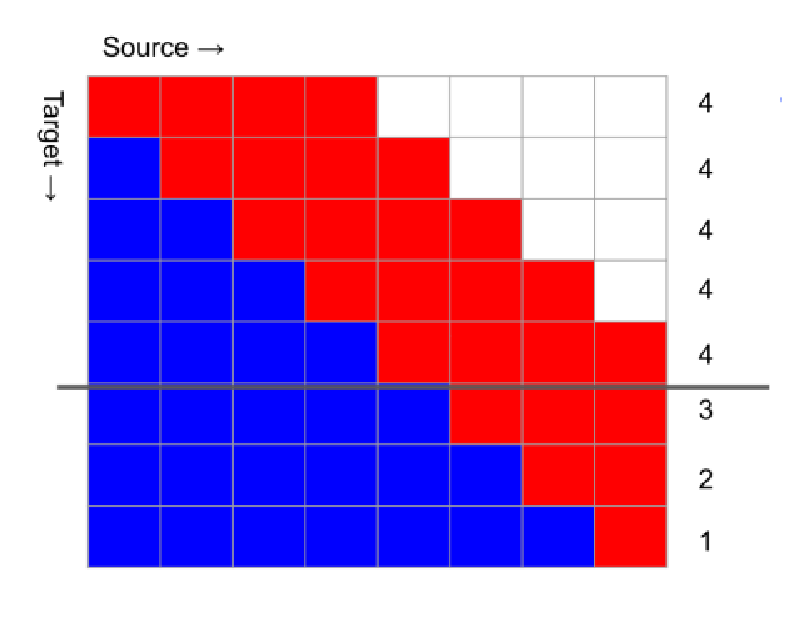
\includegraphics[width=\linewidth]{figures/AL}
  \caption*{AL}
\endminipage\hfill
\minipage{0.47\textwidth}
  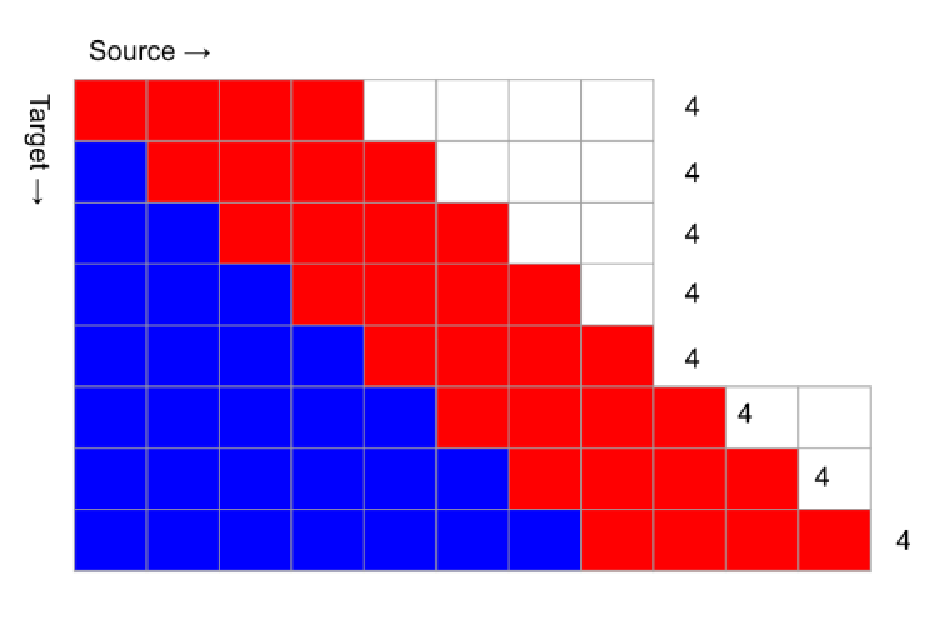
\includegraphics[width=\linewidth]{figures/DAL}
  \caption*{DAL}
\endminipage
\end{figure}

%%%%%%%%%%%%%%%%%%%%%%%%%%%%%%%%%
% RESULTS: LIST OF SYSTEMS
%%%%%%%%%%%%%%%%%%%%%%%%%%%%%%%%%
\cp
\section{Results}
\vspace*{10mm}
\begin{itemize}
	\item \textit{Baseline}: X5Gon system trained in 2019
\end{itemize}
\vspace*{-10mm}
\subsection*{Offline MT Systems}
\vspace*{5mm}
\subsubsection*{General Domain}
\vspace*{5mm}
\begin{table}[!htp]
\centering
\scalebox{0.8}{
\begin{tabular}{r||ccc|ccccc}
Name	& \multicolumn{3}{c}{Filtering}	& \multicolumn{5}{c}{Processing} \\
			&	Langid	& Length 	& Ratio		&	Apostrophes	& Tokenize	& Truecase	& BPE	& SPM 	\\ \hline
V1			& 	-			&		-		&	-			&	-				&	X				&	X				&	X		&		-	\\
V2			& 	X			&	<150		&	1.5		&	-				&	X				&	X				&	X		&	-		\\
V3			& 	X			&	<150		&	1.5		&	X				&	-				&	X				&	-		&	X		\\
\end{tabular}
}
\end{table}
\vspace*{-10mm}
\subsubsection*{In-Domain}
\begin{itemize}
	\item V3-FT-CN: V3 fine-tuned on the CERN News corpus
	\item V3-FT-BT: V3 fine-tuned on 50K backtranslations of the CDS corpus
	\item V4: V3 + backtranslations
\end{itemize}

%%%%%%%%%%%%%%%%%%%%%%%%%%%%%%%%%
% RESULTS: GENERAL DOMAIN
%%%%%%%%%%%%%%%%%%%%%%%%%%%%%%%%%

\cp
\section*{Results}
\vspace*{10mm}
\subsection*{General Domain Evaluation}
\vspace*{5mm}
\setlength{\tabcolsep}{12pt}
\begin{table}[H]
\centering
\scalebox{1}{
\begin{tabular}{l|cc}
	System					&	\multicolumn{2}{|c}{BLEU}	\\
								&	WMT13			&	WMT14			\\	\hline
	X5Gon					&34.7				&39.4				\\
	V1							&\textbf{35.1}	&39.2				\\
	V2							&\textbf{35.1}	&\textbf{39.5}	\\
	V3							&34.8				&39.3				\\
	V4							&34.6				&39.1				\\
\end{tabular}
}
\end{table}
\subsection*{In-Domain Evaluation}
\vspace*{5mm}
\begin{table}[!ht]
\centering
\scalebox{1}{
\begin{tabular}{l|cc}
	System					&	\multicolumn{2}{|c}{BLEU}	\\
								&	CN21			&	CN22			\\	\hline
	X5Gon					&35.3				&36.8				\\
	V3							&\textbf{36.9}	&\textbf{38.6}	\\
	V4							&36.6				&38.2				\\
\end{tabular}
}
\end{table}

%%%%%%%%%%%%%%%%%%%%%%%%%%%%%%%%%
% RESULTS: DOMAIN ADAPTATION
%%%%%%%%%%%%%%%%%%%%%%%%%%%%%%%%%

\cp
\section*{Results}
\vspace*{10mm}
\subsection*{Fine-Tuning}
\vspace{-5mm}
\begin{figure}[htp]
\begin{subfigure}{.5\textwidth}
\centering
\includegraphics[trim=1cm 1.5cm 1cm 3cm, scale=0.5, clip]{figures/bleu-checkpoints-finetuning-cernnews}
\end{subfigure}
\begin{subfigure}{.5\textwidth}
\centering
\includegraphics[trim=1cm 1.5cm 1cm 3cm, scale=0.5, clip]{figures/bleu-checkpoints-finetuning-backtranslation}
\end{subfigure}
\end{figure}

\begin{itemize}
	\item Best model: V3 fine-tuned using CERN News with 1000 updates
\end{itemize}
\begin{table}[ht]
\centering
\scalebox{1}{
\begin{tabular}{l|ccc}
Corpus		& BLEU (WMT14)	& BLEU (CN22)	\\ \hline
X5Gon 		&	39.4					&	36.8				\\
V3-FT-CN	&	31.7					&	42.9 				\\ 
\end{tabular}
}
\end{table}

%%%%%%%%%%%%%%%%%%%%%%%%%%%%%%%%%
% RESULTS: SIMULTANEOUS TRANSLATION
%%%%%%%%%%%%%%%%%%%%%%%%%%%%%%%%%

\cp
\section*{Results}
\vspace*{10mm}
\subsection*{Streaming MT}
\vspace{-7.5mm}
\begin{figure}[htp]
\begin{subfigure}{.5\textwidth}
\centering
\includegraphics[trim=1cm 1cm 1cm 1.5cm, scale=0.85, clip]{figures/bleu-latency-wmt13}
\end{subfigure}
\begin{subfigure}{.5\textwidth}
\centering
\includegraphics[trim=1cm 1cm 1cm 1.5cm, scale=0.85, clip]{figures/bleu-latency-cn21}
\end{subfigure}
\end{figure}
\begin{itemize}
	\item Selected models: V3 Multi-Path Wait-$k$ with $k \geq 7$
\end{itemize}
\begin{table}[ht]
\centering
\scalebox{1}{
\begin{tabular}{l||c||cc}
Corpus		& BLEU &	 AL	& 	DAL 	\\ \hline
WMT14		&	33.8 	&	5.9	&	7.1	\\
CN22		&	30.9 	&	5.5	&	7.1	\\ 
\end{tabular}
}
\end{table}

%%%%%%%%%%%%%%%%%%%%%%%%%%%%%%%%%
% CONCLUSION & FUTURE WORK
%%%%%%%%%%%%%%%%%%%%%%%%%%%%%%%%%

\cp
\section{Conclusions}
\vspace*{10mm}
\subsection*{Achieved Goals}
\begin{itemize}\itemsep=5mm
	\item Studied SOTA for offline and simultaneous MT, domain adaptation and automatic evaluation
	\item Leveraged current tools used for MT research to develop various MT systems
	\item Refined the data processing pipeline and improved MT system performance
	\item Developed in-domain MT systems, improving the baseline by a relative 11\%
	\item Developed high-accuracy and low-latency simultaneous MT systems for streaming applications
\end{itemize}

\subsection*{Future work}
\begin{itemize}\itemsep=5mm
	\item Deploy the MT systems in CERN's network
	\item Carry out domain adaptation for simultaneous MT systems
	\item Explore:
	\begin{itemize}
		\item Domain adaptation beyond fine-tuning with \textit{adapter layers}
		\item Adaptive policies for simultaneous translation by identifying \textit{meaningful units}
	\end{itemize}	
\end{itemize}

%%%%%%%%%%%%%%%%%%%%%%%%%%%%%%%%%
% SAME AS START
%%%%%%%%%%%%%%%%%%%%%%%%%%%%%%%%%
\cp
\thispagestyle{empty}

\begin{center}

\centerline{\includegraphics[height=0.15\textheight]{figures/UPV-logo}}

\rule{0mm}{20mm}
\Large{\setstretch{1.5}\Large\textbf{\color{darkred}\title}}

\rule{0mm}{30mm}
{\normalsize \color{greyblue}\author}

\newcolumntype{Y}{>{\centering\arraybackslash}X}
\rule{0mm}{0mm}
\begin{table}[ht!]
    \begin{tabularx}{\textwidth}{YY}
        \small \color{greyblue} Jorge Civera Saiz & \small \color{greyblue} Javier Iranzo Sánchez\\
    \end{tabularx}
\end{table}

\end{center}

\centerline{\includegraphics[height=0.12\textheight]{figures/MLLP_Brand} \qquad \qquad \includegraphics[height=0.15\textheight]{figures/vrain.png}}

\normalsize\small
\vspace{10mm}

\centerline{\today}
\vfill

%%%%%%%%%%%%%%%%%%%%%%%%%%%%%%%%%%%%%%%%%%%%%%%%%%%%%%%%%%%%%%%%%%%%%%%%%%%%%%%%%%%%%%%%%%%%%%%%%%
%%%%%%%%%%%%%%%%%%%%%%%%%%%%%%%%%%%%%%%%%%%%%%%%%%%%%%%%%%%%%%%%%%%%%%%%%%%%%%%%%%%%%%%%%%%%%%%%%%
%%%%%%%%%%%%%%%%%%%%%%%%%%%%%%%%%%%%%%%%%%%%%%%%%%%%%%%%%%%%%%%%%%%%%%%%%%%%%%%%%%%%%%%%%%%%%%%%%%

%%%%%%%%%%%%%%%%%%%%%%%%%%%%%%%%%
% ADDITIONAL MATERIAL: IBM Model 1
%%%%%%%%%%%%%%%%%%%%%%%%%%%%%%%%%
\cp
\thispagestyle{empty}
\section*{Appendix}
\vspace*{10mm}
\subsection*{IBM Model 1}
\begin{figure}[!htp]
\centering
\includegraphics[trim=4.5cm 10cm 3.5cm 10cm, scale=1.6, clip]{figures/ibm1}
\end{figure}

%%%%%%%%%%%%%%%%%%%%%%%%%%%%%%%%%
% ADDITIONAL MATERIAL: TRANSFORMER ENCODER-DECODER
%%%%%%%%%%%%%%%%%%%%%%%%%%%%%%%%%
\cp
\thispagestyle{empty}
\section*{Appendix}
\vspace*{10mm}
\subsection*{Transformer Encoder-Decoder}
\vspace*{-15mm}

\begin{figure}[!htp]
\centering
\includegraphics[trim=4cm 8cm 3cm 8cm, scale=1.35, clip]{figures/transformer_encoder_decoder}
\end{figure}

%%%%%%%%%%%%%%%%%%%%%%%%%%%%%%%%%
% ADDITIONAL MATERIAL: BEAM SEARCH
%%%%%%%%%%%%%%%%%%%%%%%%%%%%%%%%%
\cp
\thispagestyle{empty}
\section*{Appendix}
\vspace*{10mm}
\subsection*{Beam Search}

\begin{figure}[!htp]
\centering
\includegraphics[trim=4cm 10cm 4cm 10cm, scale=1.7, clip]{figures/beam-search}
\end{figure}

%%%%%%%%%%%%%%%%%%%%%%%%%%%%%%%%%
% ADDITIONAL MATERIAL: BLEU TER CHRF
%%%%%%%%%%%%%%%%%%%%%%%%%%%%%%%%%
\cp
\thispagestyle{empty}
\section*{Appendix}
\vspace*{10mm}
\subsection*{Quality Evaluation}
\vspace*{5mm}
\subsubsection*{BLEU}
\begin{equation}\nonumber
	BLEU(4) = BrevityPenalty \times AveragePrecision(4) 
\end{equation}

\begin{equation}\nonumber
	BrevityPenalty = \left\{
		 \begin{array}{ll}
		 	1 & \quad |output| > |reference|	\\
		 	\exp\bigg (1 - \frac{|output|}{|reference|}\bigg) & \quad |output| \leq |reference|
   		 \end{array}
    \right.	
\end{equation}

\begin{equation}\nonumber
	AveragePrecision(N) = \frac{1}{N} \sum_{n=1}^N log p_n, \qquad 	p_n = \frac{\mbox{matching n-grams}}{\mbox{total n-grams in output}}
\end{equation}

\subsubsection*{chrF}
 \begin{equation}\nonumber
 	chrF \beta = (1 + \beta)^2 \frac{chrP \times chrR}{\beta^2 \times chrP + chrR}
 \end{equation}
\subsubsection*{TER}
\begin{equation}\nonumber
	TER = \frac{\mbox{word-level edit distance}}{|\mbox{reference}|}
\end{equation}

%%%%%%%%%%%%%%%%%%%%%%%%%%%%%%%%%
% ADDITIONAL MATERIAL: WAIT-K
%%%%%%%%%%%%%%%%%%%%%%%%%%%%%%%%%
\cp
\thispagestyle{empty}
\section*{Appendix}
\vspace*{10mm}
\subsection*{Simultaneous Translation}
\vspace*{5mm}
\begin{itemize}
	\item $g(i)$ is the number of source tokens read when writing a translation at position $i$.
\end{itemize}
\subsubsection*{Wait-$k$}
\begin{equation}\nonumber
	g_{\text{wait}-k}(i) = \floor*{k+\frac{i-1}{\gamma}}, \qquad	\gamma=\mathbb{E}\big[\gamma_n\big], 	\qquad \gamma_n = \frac{|\mathbf{y}_n|}{| \mathbf{x}_n|}.
\end{equation}

\subsubsection*{Multi-Path Wait-$k$}
For one  wait-$k$ path $\mathbf{z}_{<i}^k$:
\begin{equation}\nonumber
p(\mathbf{y} \mid \mathbf{x}, \mathbf{z}^k) = \prod_i p(y_i \mid \mathbf{x}_{\leq \mathbf{z}_i^k}, \mathbf{y}_{<i}, \mathbf{z}_{<i}^k).
\end{equation}\nonumber
We optimize over multiple wait-$k$ paths:
\begin{equation}\nonumber
\mathbb{E}_K[p(\mathbf{y} \mid \mathbf{x}, \mathbf{z}^k)] \approx \prod_{k \sim \mathcal{U}(K)} p(\mathbf{y} \mid \mathbf{x}, \mathbf{z}^k).
\end{equation}

%%%%%%%%%%%%%%%%%%%%%%%%%%%%%%%%%
% ADDITIONAL MATERIAL: AP, AL, DAL
%%%%%%%%%%%%%%%%%%%%%%%%%%%%%%%%%

\cp
\thispagestyle{empty}
\section*{Appendix}
\vspace*{10mm}
\subsection*{}
\vspace*{5mm}
\subsubsection*{Average Proportion}
\begin{equation}\nonumber
	AP = \frac{1}{|\mathbf{x}| |\mathbf{y}|} \sum_{i=1}^{\mathbf{y}} g(i)
\end{equation}

\subsubsection*{Average Lagging}
\begin{equation}\nonumber
	AL_g = \frac{1}{\tau} \sum_{i=1}^{\tau} \bigg(g(i) - \frac{i - 1}{\gamma}\bigg), \qquad \tau = \tau_g(| \mathbf{x} |) = \min_{i : g(i) = |\mathbf{x}|} i
\end{equation}

\subsubsection*{Differentiable Average Lagging}
\begin{equation}\nonumber
	DAL_d = \frac{1}{| \mathbf{y} |} \sum_{i=1}^{| \mathbf{y} |} \bigg(g_d\prime(i) - (i-1)d \bigg), \qquad d = \frac{1}{\gamma} = \frac{| \mathbf{x} |}{| \mathbf{y} |}
\end{equation}
\begin{equation}\nonumber
g_d\prime(i) = \left\{
		\begin{array}{ll}
			g(i) & \quad i = 1\\
			\max \bigg( g(i), g_d\prime(i-1)+d\bigg) & \quad i > 1\\
		\end{array}
	\right.
\end{equation}

%%%%%%%%%%%%%%%%%%%%%%%%%%%%%%%%%
% ADDITIONAL MATERIAL: EXPERIMENTAL SETUP
%%%%%%%%%%%%%%%%%%%%%%%%%%%%%%%%%
\cp
\thispagestyle{empty}
\section*{Appendix}
\vspace*{10mm}
\subsection*{Experimental Setup}
\vspace*{-25mm}

\begin{figure}[!htp]
\centering
\includegraphics[trim=5cm 17.2cm 5cm 2.5cm, scale=1.75, clip]{figures/experimental_setup}
\end{figure}

%%%%%%%%%%%%%%%%%%%%%%%%%%%%%%%%%
% ADDITIONAL MATERIAL: ALL MT SYSTEMS
%%%%%%%%%%%%%%%%%%%%%%%%%%%%%%%%%

\cp
\thispagestyle{empty}
\section*{Appendix}
\vspace*{10mm}
\begin{itemize}
	\item \textit{Baseline}: X5Gon system trained in 2019
\end{itemize}
\vspace*{-10mm}
\subsection*{Offline MT Systems}
\subsubsection*{General Domain}
\begin{table}[!htp]
\centering
\scalebox{0.8}{
\begin{tabular}{r||ccc|ccccc}
Name	& \multicolumn{3}{c}{Filtering}	& \multicolumn{5}{c}{Processing} \\
			&	Langid	& Length 	& Ratio		&	Apostrophes	& Tokenize	& Truecase	& BPE	& SPM 	\\ \hline
V1			& 	-			&		-		&	-			&	-				&	X				&	X				&	X		&		-	\\
V2			& 	X			&	<150		&	1.5		&	-				&	X				&	X				&	X		&	-		\\
V3			& 	X			&	<150		&	1.5		&	X				&	-				&	X				&	-		&	X		\\
%V4			& 	X			&	<250		&	1.5		&	X				&					&	X				&			&	X		\\ 				
\end{tabular}
}
\end{table}
\vspace*{-15mm}
\subsubsection*{In-Domain}
\begin{itemize}
	\item V3-FT-CN: V3 fine-tuned on the CERN News corpus
	\item V3-FT-BT: V3 fine-tuned on 50K backtranslations of the CDS corpus
	\item V4: V3 + backtranslations
\end{itemize}
\vspace*{-10mm}
\subsection*{Streaming MT Systems}
\begin{itemize}
	\item V3-TT: Test-Time Wait-$k$ applied to V3
	\item V3-MP: Multi-Path Wait-$k$ training with same data processing as V3
\end{itemize}

\end{document}
